\chapter{Loss Function}
Una \textbf{funzione di costo} (o loss function) è un elemento fondamentale nel Deep Learning, perché misura \textit{quanto è sbagliata la predizione di un modello} rispetto ai valori reali. L'obiettivo dell'apprendimento automatico è quello di minimizzare questa funzione, in modo che il modello faccia previsioni più accurate, la misurazione delle funzioni di costo, come abbiamo già detto in precedenza è fondamentale per un criterio valutativo, ma anche per effetuarvi la Backpropagation nelle reti neurali.
\section{MSE Loss}
La funzione \texttt{nn.MSELoss()} calcola l'errore quadratico medio (MSE) tra le predizioni e i valori target, questa tipologia di funzione di costo utilizza la L2 Norm:
\begin{equation}
L = \frac{1}{N} \sum_{i=1}^{N} (x_i - y_i)^2
\end{equation}
Questa funzione di costo è sensibile agli outlier poiché gli errori vengono elevati al quadrato.
\section{L1 Loss}
La \texttt{nn.L1Loss()} invece misura l'errore assoluto medio (MAE) tra le predizioni e i valori target, questa tipologia di funzione di costo utilizza la L1 Norm:
\begin{equation}
L = \frac{1}{N} \sum_{i=1}^{N} |x_i - y_i|
\end{equation}
Questa funzione di costo, rispetto alla precedente risulta essere più robusta agli outlier.
\section{L1 vs L2}
Ci si è chiesti pertanto quale delle due è maggiormente corretto utilizzare, si è giunti a delle considerazioni sulla base di visioni sperimentali. Infatti seguono due diversi comportamenti. Si è mostrato come il comportamento ottenuto con L2, qui tutti i valori vengono distribuiti uniformemente, mentre con L1 i risultati sono leggermente più netti. Questa caratteristica può essere visualizzata attraverso l'utilizzo di modelli di computer vision, infatti si è potuto verificare sperimentalmente come in effetti L1 sia migliore quando ci sono delle immagini più spigolose, diversamente otteniamo un risultato migliore con L2 in immagini che risultano essere più morbide nelle loro forme (Figura~\ref{fig:l1l2diff}).

\begin{figure}
    \centering
    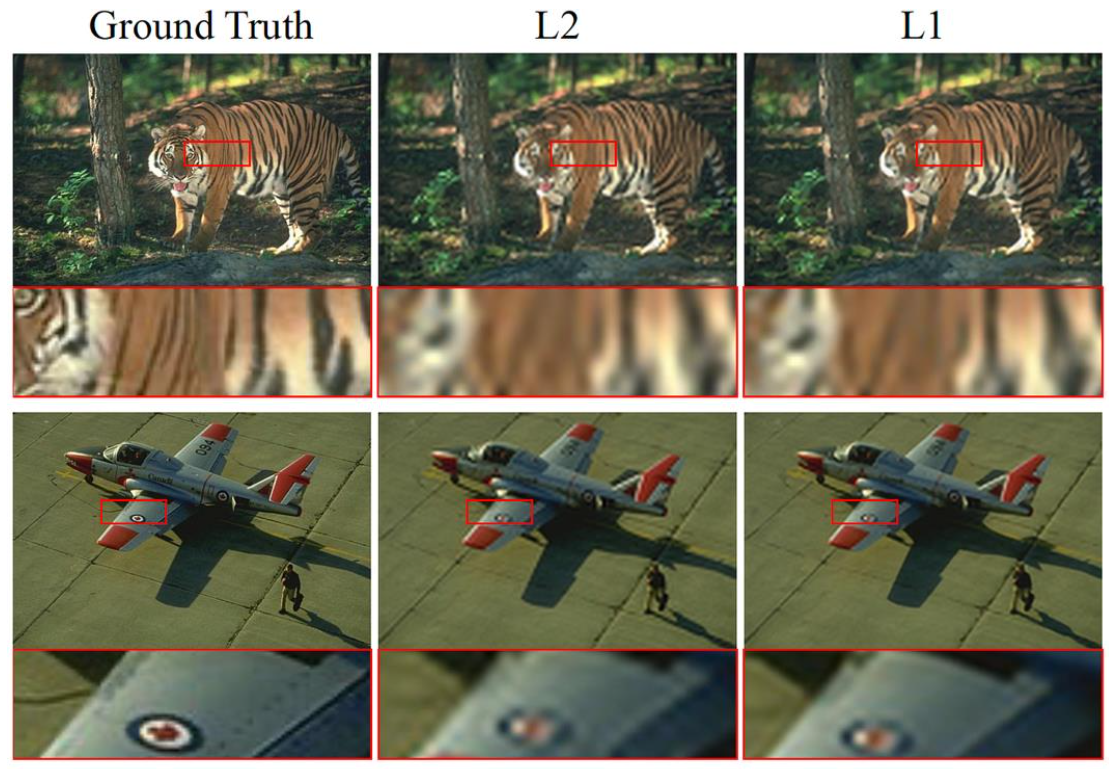
\includegraphics[width=0.75\linewidth]{figure/L1andL2.png}
    \caption{Utilizzando un modello di computer vision possiamo notare come è più accurata la norma 2 per figure meno spigolose, come quella della tigre, differentemente per l'immagine in cui vi è l'aereo la norma 1 è migliore poiché l'immagine risulta più spigolosa.}
    \label{fig:l1l2diff}
\end{figure}

\section{Smooth L1 Loss}
Per far sì che si trovi un equilibrio fra le due si è optato per creare una combinazione tra L1 e MSE per gestire gli outlier al meglio e la stabilità numerica, implementando la Smooth L1 Loss:
\begin{equation}
L(x, y) = \begin{cases} 
\frac{1}{2} (x - y)^2, & \text{se } |x - y| < 1 \\
|x - y| - \frac{1}{2}, & \text{altrimenti}
\end{cases}
\end{equation}

Qui pertanto abbiamo una combinazione delle due precedenti, in alcuni casi viene utilizzata la norma 2 in altri viene applicata la norma 1, favorendo un'ottimizzazione più netta.
\section{Negative Log Likelihood Loss}
La Negative Log Likelihood Loss (NLL Loss) è una funzione di costo comunemente usata nei problemi di classificazione multi-classe, soprattutto quando l'output del modello è espresso in log-probabilità (tramite LogSoftMax). Quando il dataset risulta essere sbilanciato, la NLL Loss tende a favorire le classi più frequenti, portando il modello a ignorare quelle meno rappresentate. Per risolvere questo problema, si può modificare la NLL Loss aggiungendo pesi per ogni classe. Essa è definita come segue, la seguente equazione la mostra considerando quella media basata su N esempi:

\begin{equation}
    L = -\frac{1}{N}\sum^{N}_{i=1}\log P(y_i|x_i)
\end{equation}

\subsection{Problema delle classi sbilanciate}
Se un dataset risulta essere sbilanciato, il modello tenderà a imparare a minimizzare la loss predicendo sempre la classe più frequente.

\begin{Esempio}
    Se il dataset ha 90\% di classe A e 10\% di classe B, il modello potrebbe semplicemente predire sempre classe A per minimizzare la loss, portando a un'accuratezza apparente alta ma con prestazioni pessime per la classe B.
\end{Esempio}

La soluzione a questa possibilità, è quella di aggiungere ulteriori pesi alle classi nella NLL Loss. Il bilancaimento viene effettuato nel seguente modo:

\begin{equation}
    L = -\frac{1}{N}\sum^{N}_{i=1}w_{y_i}\log P(y_i|x_i)
\end{equation}

Introducendo molto semplicemente un peso $w_{y_i}$ a ogni classe. Valorizzando in maniera migliore la classe minoritaria, che altrimenti verrebbe inevitabilmente schiacciata dall'altra allenando dunque il nostro modello nella maniera scorretta. Aumentare i pesi però non è la stessa cosa di avere un dataset bilanciato, pertanto è necessario chiedersi quali potrebbero essere altre soluzioni che potremmo adottare per poter bilanciare i dati.

\section{Cross Entropy Loss}
La funzione \texttt{nn.CrossEntropyLoss()} combina \texttt{LogSoftmax} e \texttt{NLLLoss} in un'unica funzione ed è la più utilizzata nei problemi di classificazione multi-classe. La perdita di entropia incrociata è definita come:
\begin{equation}
L = - \sum_{i=1}^{N} \sum_{j=1}^{C} y_{i,j} \log(\hat{y}_{i,j})
\end{equation}
dove:
\begin{itemize}
    \item $C$ è il numero di classi,
    \item $y_{i,j}$ è 1 se l'osservazione $i$ appartiene alla classe $j$, altrimenti è 0,
    \item $\hat{y}_{i,j}$ è la probabilità predetta per la classe $j$.
\end{itemize}
L'entropia incrociata permette di misurare la distanza tra due distribuzioni di probabilità: quella vera dei dati e quella predetta dal modello. Più le due distribuzioni sono simili, più bassa è la perdita. Un valore alto della perdita indica che le probabilità predette si discostano fortemente dai valori reali. Un aspetto cruciale dell'entropia incrociata è la sua connessione con la \textit{divergenza di Kullback-Leibler} (KL). La KL-divergence misura quanto una distribuzione differisce da un'altra e può essere espressa come:
\begin{equation}
D_{KL}(P||Q) = \sum_{i} P(i) \log \frac{P(i)}{Q(i)}
\end{equation}
dove $P$ rappresenta la distribuzione reale e $Q$ quella predetta. La cross-entropy include implicitamente questa metrica, motivo per cui è così efficace nei problemi di classificazione.

\section{Adaptive Log Softmax with Loss}
Quando si hanno problemi con molte classi, l'uso di una softmax standard può essere inefficiente. Per questo motivo si introduce \texttt{nn.AdaptiveLogSoftmaxWithLoss()}, che suddivide le classi in gruppi gerarchici e riduce il costo computazionale.

\section{Binary Cross Entropy Loss}
Per problemi di classificazione binaria, MSE non è ideale perché non gestisce correttamente la probabilità logaritmica. Si introduce quindi la funzione \texttt{nn.BCELoss()}:
\begin{equation}
L = - \frac{1}{N} \sum_{i=1}^{N} -w_i\left[y_i \log({x}_i) + (1 - y_i) \log(1 - x_i) \right]
\end{equation}
Questa funzione penalizza maggiormente le previsioni errate con alta confidenza, risultando più efficace rispetto a MSE per la classificazione.

\section{Kullback-Leibler Divergence Loss}
BCELoss assume che la distribuzione target sia binaria, ma a volte vogliamo misurare quanto una distribuzione di probabilità predetta si discosti da quella reale. Per questo si usa la KL Divergence:
\begin{equation}
D_{KL}(P||Q) = \sum_{i} P(i) \log \frac{P(i)}{Q(i)}
\end{equation}
Questa misura è utile per modelli probabilistici come le reti neurali bayesiane.

\section{BCE Loss with Logits}
Un problema della BCE standard è che richiede l'utilizzo della funzione sigmoide in maniera separata, questo fattore potrebbe causare instabilità numerica. Per risolvere questo problema pertanto, la \texttt{nn.BCEWithLogitsLoss()} incorpora direttamente la sigmoide nella perdita.
\begin{equation}
    L = - \frac{1}{N} \sum_{i=1}^{N} -w_i\left[y_i \log(\sigma({x}_i)) + (1 - y_i) \log(1 - \sigma({x}_i) \right]
\end{equation}

\section{Hinge Embedding Loss}
Quando si lavora con problemi di similarità (es. metric learning), vogliamo una funzione di costo che enfatizzi la distanza tra esempi simili e dissimili. \texttt{nn.HingeEmbeddingLoss()} è utile in questi casi. Infatti se la nostra distanza è inferiore a un certo limite otterrò la selezione all'interno di un valore dando come risultato un valore, alternativamente avrò come esito un altro.

\section{Margin Ranking Loss}
Simile alla Hinge Loss, ma si usa in compiti di ranking dove dobbiamo garantire che un elemento corretto abbia punteggio più alto rispetto a un elemento errato, questo ci permette al nostro sistema di ordinare qualcosa al meglio.
\begin{equation}
    L = \max(-y\,(x_1-x_2)+\text{margin},\,0) 
\end{equation}

\section{Triplet Margin Loss}
Per migliorare la distinzione tra classi, \texttt{nn.TripletMarginLoss()} è ciò che viene utilizzato, questa confronta un'ancora, con un esempio positivo e uno negativo, questo ci permette anche di considerare più di due singole categorie:
\begin{equation}
L = \max(0, d(a, p) - d(a, n) + \text{margin})
\end{equation}
Questa funzione risulta essere cruciale per l'apprendimento di embedding robusti, come nel riconoscimento facciale.

\section{Soft Margin Loss}
Una variante della Hinge Loss che introduce una penalità logistica per evitare margini rigidi:
\begin{equation}
L = \sum_{i=1}^{N} \log(1 + e^{-y_i x_i})
\end{equation}

Questa funzione di costo non fa altro che integrare la funzione di softmax, a quella logistica, volendo fare in modo che i valori positivi siano più vicini fra loro e spingeranno i valori negativi lontani aggiungendo un decadimento esponenziale alla funzione di costo.

\section{Multi-Class Hinge Loss}
Quando abbiamo più di due classi, una semplice Hinge Loss non è sufficiente. \texttt{nn.MultiLabelMarginLoss()} estende il concetto a problemi multi-classe. 

\section{Cosine Embedding Loss}
Giungiamo ora all'ultima funzione di costo, nel nostro caso partiamo prendendo in considerazione un esempio partendo da delle frasi, immaginiamo che vogliamo creare una situazione in cui le frasi con lo stesso significato, possano essere legate, e se avessimo diverse frasi vogliamo trovare un modo per valutare se stanno parlando della stessa cosa o meno. Sicuramente se abbiamo due frasi diverse verranno poste in posizioni diverse nel nostro spazio latente, anche se sono leggermente diverse e parlano dello stesso contesto. Tuttavia se abbiamo la necessità di unificarle, rischiamo di perdere informazioni appiattendo la varietà di linguaggio basata su tono, espressività, gergo, ecc\dots
\begin{figure}[h]
    \centering
    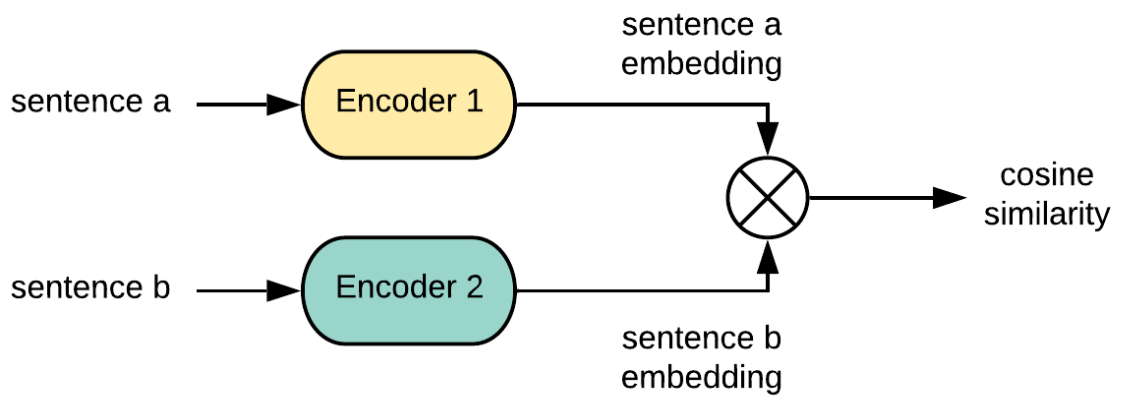
\includegraphics[width=0.75\linewidth]{figure/CosineSim.png}
    \caption{Rappresentazione di come che vorrei trattare due frasi per determinarne la loro similarità}
    \label{fig:coSim}
\end{figure}
Ciò che i ricercatori sono riusciti a capire che due parole seguono lo stesso vettore, sebbene siano leggermente differenti, possiamo fare ciò attraverso la \textbf{Cosine similarity}. Ossia si calcola il coseno dell'angolo compreso fra due vettori. Se i due vettori sono uguali fra loro la risposta sarà zero differentemente non lo sarà.
\begin{Osservazione}
    Se due vettori sono completamente diversi fra loro, idealmente i due vettori saranno posizionati ortogonalmente fra loro.
\end{Osservazione}
    
Per misurare la similarità tra vettori in uno spazio di embedding, si usa la \texttt{nn.CosineEmbeddingLoss()}:
\begin{equation}
L = \begin{cases} 
1 - \cos(x_1, x_2), & \text{se } y = 1 \\
\max(0, \cos(x_1, x_2) - \text{margin}), & \text{se } y = -1
\end{cases}
\end{equation}
\\
Questa funzione risulta essere fondamentale nei sistemi di retrieval e riconoscimento facciale.